% VLDB template version of 2020-03-05 enhances the ACM template, version 1.7.0:
% https://www.acm.org/publications/proceedings-template
% The ACM Latex guide provides further information about the ACM template

\documentclass{article}
\usepackage{listings}
\usepackage[margin=20mm]{geometry}
\usepackage{graphicx}
\usepackage{amsfonts}
\usepackage{amsmath}
\usepackage{physics}
\usepackage{parskip}
\usepackage{enumitem}
\usepackage{cancel}

%% The following content must be adapted for the final version
% paper-specific
\newcommand\vldbdoi{XX.XX/XXX.XX}
\newcommand\vldbpages{XXX-XXX}
% issue-specific
\newcommand\vldbvolume{14}
\newcommand\vldbissue{1}
\newcommand\vldbyear{2020}
% should be fine as it is
\newcommand\vldbauthors{\authors}
\newcommand\vldbtitle{\shorttitle} 
% leave empty if no availability url should be set
\newcommand\vldbavailabilityurl{http://vldb.org/pvldb/format_vol14.html}

\newcommand\oname\operatorname

\newtheorem{theorem}{Teor.}
\newtheorem{definition}{Def.}
\newtheorem{example}{Ej.}
\newtheorem{excercise}{Ejer.}

\begin{document}

% Note to self:
%   "It is never possible to expose anyone to both treatments, and therefore statistical inference would still be needed to asses the \textit{causal inference}.

\textbf{Ex. 1.12.1: }Conditional probability: suppose that if $\theta=1$, then $y$ has a normal distribution with mean $1$ and standard deviation $\sigma$, and if $\theta=2$, then $y$ has a normal distribution with mean $2$ and standard deviation $\sigma$. Also, suppose $\oname{Pr}(\theta=1)=0.5$ and $\oname{Pr}(\theta=2)=0.5$.

\begin{enumerate}[label=\alph*]
	\item For $\theta=2$, write the formula for the marginal probability density for $y$ and sketch it.
	\item What is $\oname{Pr}(\theta=1|y=1)$, again supposing $\sigma=2$?
	\item Describe how the posterior density of $\theta$ changes in shape as $\sigma$ is increased and as it is decreased.
\end{enumerate}

\textbf{Answer:}

The formula for the marginal probability is that of $\mathcal N(\theta,\,\sigma)$:
\begin{align*}
	p(y|\theta=2)&=\frac1{\sqrt{2\pi\sigma^2}}\exp\left(-\frac12\left(\frac{x-2}\sigma\right)^2\right).
\end{align*}

As for the sketch, I'm too lazy to do it. It's a bell shape, centered at $2$ and $\sigma$ being half the width at about $0.61$ height. There's an xkcd-looking MatPlotLib plot in Figure \ref{fig:1.12.1}.
\begin{figure}[h]
	\centering
	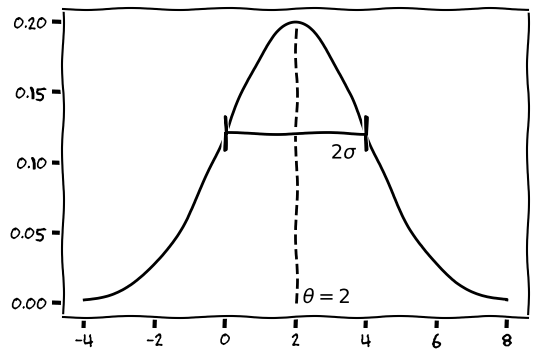
\includegraphics[width=0.4\textwidth]{Numerical/1.12.1}
	\caption{Your typical bell thingy with $\sigma=2$ and mean $2$}
	\label{fig:1.12.1}
\end{figure}

Now then,
\begin{align*}
	\oname{Pr}(\theta=1|y=1)&=\frac{\oname{Pr}(\theta=1)\oname{Pr}(y=1|\theta=1)}{\oname{Pr}(\theta=1)\oname{Pr}(y=1|\theta=1)+\oname{Pr}(\theta=2)\oname{Pr}(y=2|\theta=2)}\\
	&=\frac{0.5\cdot\frac1{\sqrt{8\pi}}}{0.5\cdot\frac1{\sqrt{8\pi}}+0.5\cdot\frac1{\sqrt{8\pi}}\exp\left(-\frac18\right)}\\
	&\approx0.53.
\end{align*}

The posterior for $\theta$ gets more homogeneous as $\sigma$ increases, and instead gets closer to $(1, 0)$ otherwise, since $\sigma$ directly defines the overlap between both likelihood functions as functions of $y$.

\end{document}
\endinput
